%%%%%%%% ForecastBench-Sim ICML Forecasting Workshop Draft %%%%%%%%%%%%%%%%

\documentclass{article}

\usepackage{microtype}
\usepackage{graphicx}
\usepackage{booktabs}
\usepackage{float}
\usepackage{hyperref}
\newcommand{\theHalgorithm}{\arabic{algorithm}}
\usepackage{icml2026_template/icml2026}
\usepackage{amsmath}
\usepackage{amssymb}
\usepackage[capitalize,noabbrev]{cleveref}

\graphicspath{{figures/}}

\icmltitlerunning{ForecastBench-Sim}

\begin{document}

\twocolumn[
  \icmltitle{ForecastBench-Sim: A Simulated-World Forecasting Benchmark}
  \icmltitlerunning{ForecastBench-Sim}

  \begin{icmlauthorlist}
    \icmlauthor{Anonymous Authors}{anon}
  \end{icmlauthorlist}

  \icmlaffiliation{anon}{Anonymous Institution}
  \icmlcorrespondingauthor{Anonymous Authors}{anonymous@anonymous.invalid}
  \icmlkeywords{forecasting, benchmark, simulated worlds, language models, probabilistic reasoning}

  \vskip 0.3in
]

\printAffiliationsAndNotice{}

\begin{abstract}
Forecasting benchmarks for general-purpose AI systems usually inherit the constraints of the real world: outcomes resolve slowly, tail events are rare, and counterfactual questions are difficult to score. We introduce ForecastBench-Sim, a simulated-world forecasting benchmark built from Freeciv game rollouts. Forecasters receive a fixed world report, a structured snapshot of the current game state, and answer binary and distributional questions about hidden future states; the benchmark then continues the simulation and scores forecasts with Brier score and CRPS. Because the world is simulated, the same setup can generate H0 report-comprehension checks, paired intervention worlds for conditional or causal questions, and resolved examples of rare or disruptive outcomes. We describe the benchmark pipeline, question families, scoring protocol, and release artifacts, and report validation slices from model evaluations and an anonymized human pilot. ForecastBench-Sim is intended to complement real-world forecasting benchmarks by providing controlled, immediately resolvable tasks for studying probabilistic reasoning under dynamic world states.
\end{abstract}

\section{Introduction}

Forecasting is a natural testbed for evaluating general-purpose AI systems: good forecasts require extracting relevant evidence, reasoning under uncertainty, and assigning calibrated probabilities to future events. Existing forecasting benchmarks such as ForecastBench are valuable, but real-world evaluation has structural limits \citep{karger2024forecastbench}. Outcomes may take weeks or months to resolve, rare events are sparsely observed, and counterfactual questions usually cannot be scored because only one world is realized.

Simulation offers a complementary route. A simulated world can preserve the basic forecasting structure---partial information, path dependence, interacting agents, and hidden future states---while giving the evaluator control over resolution and interventions. ForecastBench-Sim uses Freeciv rollouts as this substrate \citep{freeciv2026}, building on the CivRealm infrastructure for Freeciv-based AI environments \citep{qi2024civrealm}. Each task is defined by a world snapshot, a report shown to forecasters, a set of forecasting questions, and a hidden future produced by continuing the simulation.

ForecastBench-Sim supports binary event forecasts and continuous distributional forecasts over matched world reports, includes H0 checks for report comprehension, and can produce paired intervention worlds by mutating savegame state before rollout. We report compact validation results from existing model runs and a small anonymized human pilot.

\paragraph{Related work.}
Recent LLM forecasting benchmarks emphasize real-world outcome prediction with naturally occurring text and delayed resolution, including ForecastBench \citep{karger2024forecastbench}, Context is Key \citep{cik2024context}, and work on eliciting numerical predictive distributions from language models \citep{requeima2024llmprocesses}; retrieval-augmented systems can approach human-level performance on questions of this kind \citep{halawi2024forecasting}. ForecastBench-Sim instead uses a simulation-backed substrate, closer in spirit to controllable multi-agent environments such as CivRealm \citep{qi2024civrealm}. Existing causal-reasoning benchmarks for language models score formal inference over toy graphs \citep{jin2023cladder}; ForecastBench-Sim complements this by enabling matched fork-and-resolve interventional questions over rich evolving worlds, alongside work on consistency and calibration in language-model forecasting \citep{paleka2024consistency,tian2023calibration}.

\section{Benchmark Design}

\begin{figure*}[t]
  \centering
  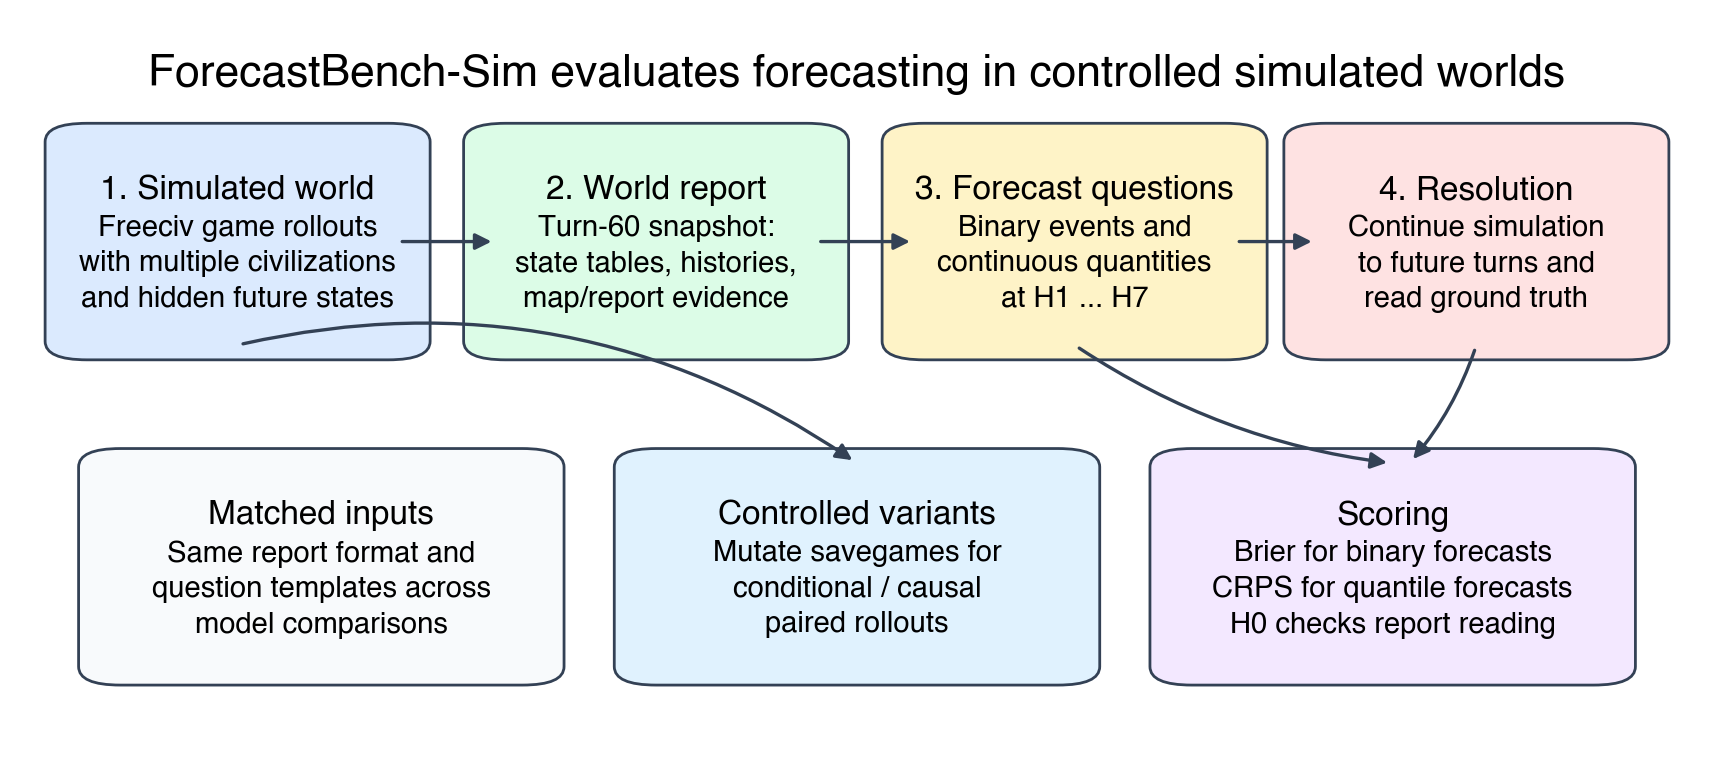
\includegraphics[width=.86\textwidth]{fig1_benchmark_schematic.png}
  \caption{ForecastBench-Sim evaluates forecasts over hidden future states in controlled simulated worlds. A fixed report is shown to forecasters; future turns are withheld until the simulation is continued and scored. The same machinery also supports paired savegame interventions for conditional or causal questions.}
  \label{fig:benchmark-schematic}
\end{figure*}

\subsection{Worlds and Reports}

ForecastBench-Sim begins from Freeciv game rollouts. Each world contains multiple civilizations with evolving cities, technology, territory, treasuries, diplomacy, and conflicts. We expose a fixed snapshot, currently at turn 60, and withhold later turns from the forecaster. The future is generated before scoring but hidden at prediction time.

The forecaster observes a world report rather than the simulator state directly. Reports are designed to be the common input surface for both language models and human participants: they summarize the turn-60 state in structured text, tables, histories, and map/report evidence. This keeps the task close to ordinary forecasting, where the forecaster sees evidence about a world rather than the answer itself, while avoiding retrieval confounds from external web search.

\begin{table}[t]
\centering
\caption{ForecastBench-Sim composition. H0 rows are report-reading checks; H1--H7 rows are forecasting tasks. T/W = templates/worlds.}
\label{tab:benchmark-composition}
\small
\begin{tabular}{lccc}
\toprule
Family & Horiz. & Qs. & T/W \\
\midrule
Binary & H1--H7 & 4,655 & 10 / 11 \\
Continuous & H1--H7 & 2,310 & 6 / 11 \\
H0 binary & H0 & 562 & 10 / 11 \\
H0 continuous & H0 & 165 & 3 / 11 \\
\bottomrule
\end{tabular}
\end{table}


\subsection{Question Families}

From each report, the benchmark generates matched forecasting questions across several future horizons. Binary questions ask whether an event or relation will hold at a later turn, and continuous questions ask for a future value of a world variable. For example, a binary question may ask whether a civilization's treasury will exceed a threshold at a future turn, while the matched continuous question asks for the treasury value itself.

Continuous questions elicit five quantiles, currently p10, p25, p50, p75, and p90. The main continuous families include city counts, technologies, and treasury values; binary templates cover a broader set of comparisons and threshold events. Forward-looking tasks use horizons H1--H7, corresponding to 30-turn increments past the turn-60 snapshot (turns 90 through 270, or roughly the second half of a typical game). H0 questions ask about the snapshot state itself and serve as comprehension checks rather than forecasting tasks.

\subsection{Scoring}

Binary forecasts are scored with Brier score \citep{brier1950verification}; continuous forecasts are scored with CRPS computed from the elicited quantiles \citep{gneiting2007proper}. We normalize CRPS by a fixed range for each template family so that cities, technologies, and treasury values can be averaged without changing the per-question scoring rule. H0 checks are reported separately because they test report reading rather than forecasting.

\section{Controlled Evaluation Affordances}

The benchmark supports three forecasting regimes, distinguished by how the conditioning event is established. Unconditional forecasts target $P(Y)$ from a fixed report; observational conditional forecasts target $P(Y \mid X)$ from natural variation across a corpus of simulated worlds; interventional forecasts target $P(Y \mid \mathrm{do}(X))$, where $X$ is set by mutating the savegame before rollout. Each regime uses the same proper scoring rules. The third is the regime that real-world forecasting benchmarks cannot ordinarily resolve, because only one history is realized; the simulator turns it into a scored question by producing a separate ground truth in each branch.

The unconditional benchmark is the closest analogue to existing real-world forecasting benchmarks. A forecaster receives a report and predicts what will later happen, without being told that any special intervention occurred. This setting supports both binary questions, scored by Brier score, and continuous questions, scored by CRPS, yielding a ForecastBench-style evaluation surface with automatic resolution and fixed prompts.

The interventional regime is the one real-world benchmarks cannot ordinarily score: the benchmark copies a savegame at the forecast turn, applies an intervention, rolls out the modified world, and scores forecasts against the intervention-world outcome. Existing pilots use two interventions, switching a civilization's government to Republic and adding 500 gold to its treasury, and reuse the same target templates under baseline and conditional framings. Across the archived nine-model slice, mean intervention gain is positive for every curated model on both pilots (+0.029 to +0.057 on Republic; +0.013 to +0.062 on +500 gold; \cref{fig:intervention-gap}). An Opus 4.5 placebo control leaves Brier nearly unchanged under null-conditional wording (0.165 vs.\ 0.169 baseline) while the real Republic conditional rises to 0.360 (\cref{fig:null-conditional}), suggesting that the response is not explained by conditional phrasing alone.

The observational regime can instead be populated by sampling a corpus of simulated worlds and measuring how often events co-occur. This slice is not yet part of the released artifact, but it remains cleanly separable from the interventional regime because the data source is a corpus rather than a forked rollout.

Finally, simulated worlds make tail-risk evaluation practical because large shocks can be sampled densely instead of waited for. As one example, a companion anonymous analysis on the same question family finds the share of treasury outcomes falling below the model's stated p10 rising to roughly 50\% by H6--H7 (\cref{fig:tail-risk}; \citealp{anonymous2026capability}).

\section{Validation Results}

We use existing model runs to check that the benchmark behaves like a forecasting evaluation rather than a report-parsing exercise. The main unconditional run contains 4,655 binary questions across 30 models and 2,310 continuous questions across 31 models. The compact leaderboard in \cref{fig:model-validation} shows the curated subset with complete coverage across the artifacts used in this paper, while preserving rank context from the larger runs.

\begin{figure}[t]
  \centering
  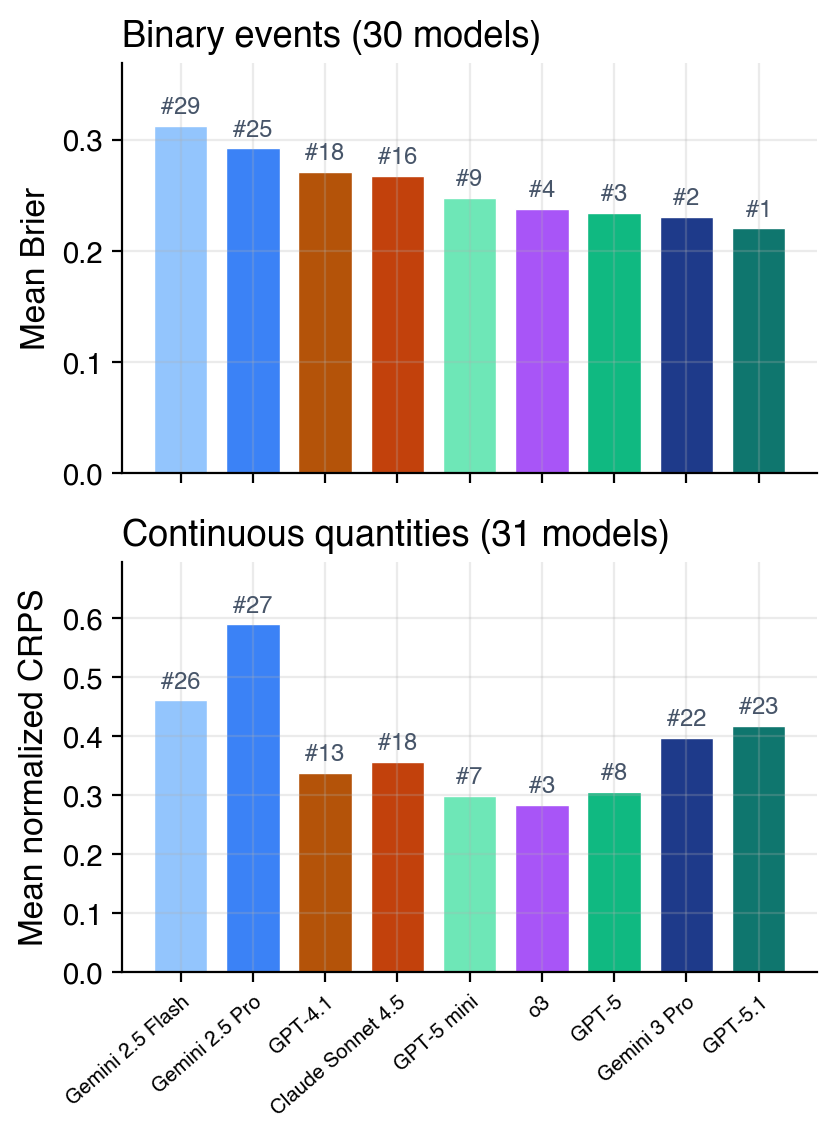
\includegraphics[width=\linewidth]{fig2_model_validation_compact.png}
  \caption{Compact validation slice for nine curated models with full coverage across model, H0, human-baseline, and intervention artifacts. Bars show average forward-looking performance; rank markers give each model's position in the larger binary or continuous run.}
  \label{fig:model-validation}
\end{figure}

The benchmark also shows meaningful horizon structure. In \cref{fig:horizon-curve}, scores vary across H1--H7. This validation result indicates that the simulated tasks contain forecastable signal and horizon-dependent uncertainty. We do not treat this workshop paper as a final model-ranking paper.

H0 checks provide a separate sanity check on the input format. The curated models score near-perfectly on H0 continuous questions and low Brier on H0 binary questions, suggesting that forward-looking errors are not primarily caused by inability to read the turn-60 reports. Detailed H0 results are in \cref{app:h0}.

Finally, the anonymized human pilot demonstrates that the same task family can be presented to people. Ten participants answered 24 continuous questions over two worlds, covering city, technology, and treasury templates at H1, H3, H4, and H6. The crowd-mean normalized CRPS is close to a uniform-bin baseline in this small pilot, so we treat it as a feasibility check and a guide for a larger human baseline rather than as a definitive model comparison; details are in \cref{app:human-pilot}.

\begin{figure}[t]
  \centering
  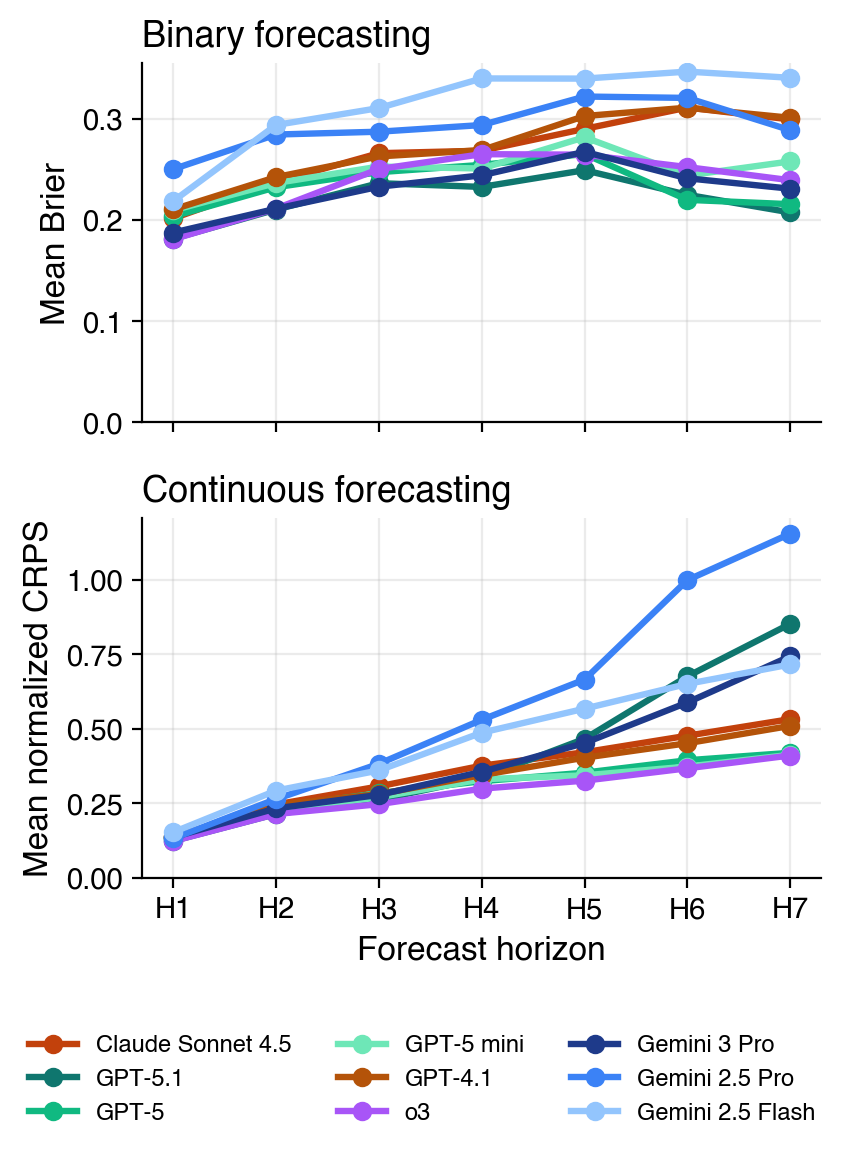
\includegraphics[width=\linewidth]{fig3_horizon_curve.png}
  \caption{ForecastBench-Sim captures horizon-dependent difficulty. Scores are averaged by horizon for the curated model set; H0 checks are omitted from the main curve because they test report comprehension rather than future forecasting.}
  \label{fig:horizon-curve}
\end{figure}

\section{Future Work}

ForecastBench-Sim currently uses Freeciv because it provides an inspectable multi-agent world with saved states and replay infrastructure, but the broader goal is a family of simulation-backed slices that plug into the same evaluation interface alongside dataset and market questions in benchmarks like ForecastBench. Different substrates would expose different forecasting skills. Generative-agent social simulators such as Concordia \citep{vezhnevets2023concordia} probe whether models can predict the behavior of other agents under social pressure. Epidemiological agent-based models would produce dense tail-risk material---outbreak surges, intervention counterfactuals, and rare cascades---without waiting for real outbreaks. Logistics, climate-resource, and bureaucratic-process simulators could play similar roles for their respective skill profiles.

A second extension changes how forecasts are scored, not where they come from. Instead of resolving a probability against a single $0/1$ outcome, the same starting world can be rolled out $N$ times under different RNG seeds and forecasts resolved against the empirical event frequency across rollouts. This converts resolution from a single noisy realization into a target close to the simulator's true generating probability---only possible because the world is simulated---while keeping Brier score and CRPS proper against the continuous target.

Two further directions are natural under the same machinery: sequential forecasting, where the report is revealed at multiple snapshots and models must update as evidence accumulates, and counterfactual coherence checks, where the same target is queried under multiple conditional framings to test whether a model's conditionals respect basic probability axioms \citep{paleka2024consistency}.

\section{Limitations}

ForecastBench-Sim is not a substitute for real-world forecasting benchmarks. Freeciv worlds are simplified and stylized, report formatting can affect both models and humans, and the current human study is only a pilot. The conditional and causal artifacts are demonstrations rather than a fully powered intervention benchmark.

\section{Conclusion}

ForecastBench-Sim is a simulated-world forecasting benchmark designed to complement real-world evaluations rather than replace them. In the current release, it contributes three main capabilities within a single forecasting interface: unconditional binary and distributional forecasting over fixed world reports, paired intervention rollouts for scored causal-conditional questions, and dense sampling of disruptive outcomes that can support tail-risk analysis with immediate resolution. We view that combination as the benchmark's main contribution: not a final empirical ranking of forecasters, but a reusable evaluation substrate on which later work can make narrower claims about calibration, causal updating, and rare-event forecasting behavior.

\clearpage
\bibliography{forecastbench_sim}
\bibliographystyle{icml2026_template/icml2026}

\clearpage
\appendix
\onecolumn

\section{H0 Comprehension Checks}
\label{app:h0}

H0 questions ask for quantities that are already present in the turn-60 report. They are not included in forward-looking scores, but they are important for interpreting those scores: a model that fails H0 may be failing to extract the report, while a model that passes H0 and fails H1--H7 is more plausibly failing at forecasting. The curated models pass this check on the continuous questions and have low binary Brier scores, so the main validation curves are not driven by obvious report-reading failures.

\begin{table}[t]
\centering
\caption{H0 comprehension checks. H0 questions are answerable from the turn-60 report and test report reading rather than future forecasting. Lower is better.}
\label{tab:h0-comprehension}
\small
\resizebox{0.78\linewidth}{!}{%
\begin{tabular}{lrrrr}
\toprule
Model & Bin. Brier & Bin. $n$ & Cont. nCRPS & Cont. $n$ \\
\midrule
Claude Sonnet 4.5 & 0.0142 & 562 & 0.0000 & 165/165 \\
GPT-5.1 & 0.0178 & 562 & 0.0008 & 165/165 \\
GPT-5 & 0.0035 & 562 & 0.0000 & 165/165 \\
GPT-5 mini & 0.0002 & 562 & 0.0004 & 165/165 \\
GPT-4.1 & 0.0276 & 562 & 0.0001 & 165/165 \\
o3 & 0.0053 & 562 & 0.0029 & 165/165 \\
Gemini 3 Pro & 0.0319 & 562 & 0.0240 & 165/165 \\
Gemini 2.5 Pro & 0.0047 & 562 & 0.0000 & 165/165 \\
Gemini 2.5 Flash & 0.0018 & 562 & 0.0000 & 165/165 \\
\bottomrule
\end{tabular}
}
\end{table}


\section{Human Pilot Details}
\label{app:human-pilot}

The anonymized pilot contains 10 participants, 24 continuous questions, and 240 individual forecasts. Participants saw two simulated-world reports and allocated probability mass across five bins for city, technology, and treasury questions at H1, H3, H4, and H6. The released data remove raw survey identifiers, timestamps, demographics, consent fields, free-text comments, and mouse/click events.

The pilot is useful for checking task feasibility and for constructing a preliminary human reference point. Mean individual normalized CRPS is 0.171, the crowd mean is 0.154, and the uniform-bin baseline is 0.152 on these 24 questions. The crowd aggregation helps relative to individual responses, but the pilot does not clearly beat the uninformed baseline. This is consistent with the study being small, general-population, and cognitively demanding; it motivates a larger and more carefully powered human baseline rather than supporting a strong human-vs-model claim.

\begin{figure}[h]
  \centering
  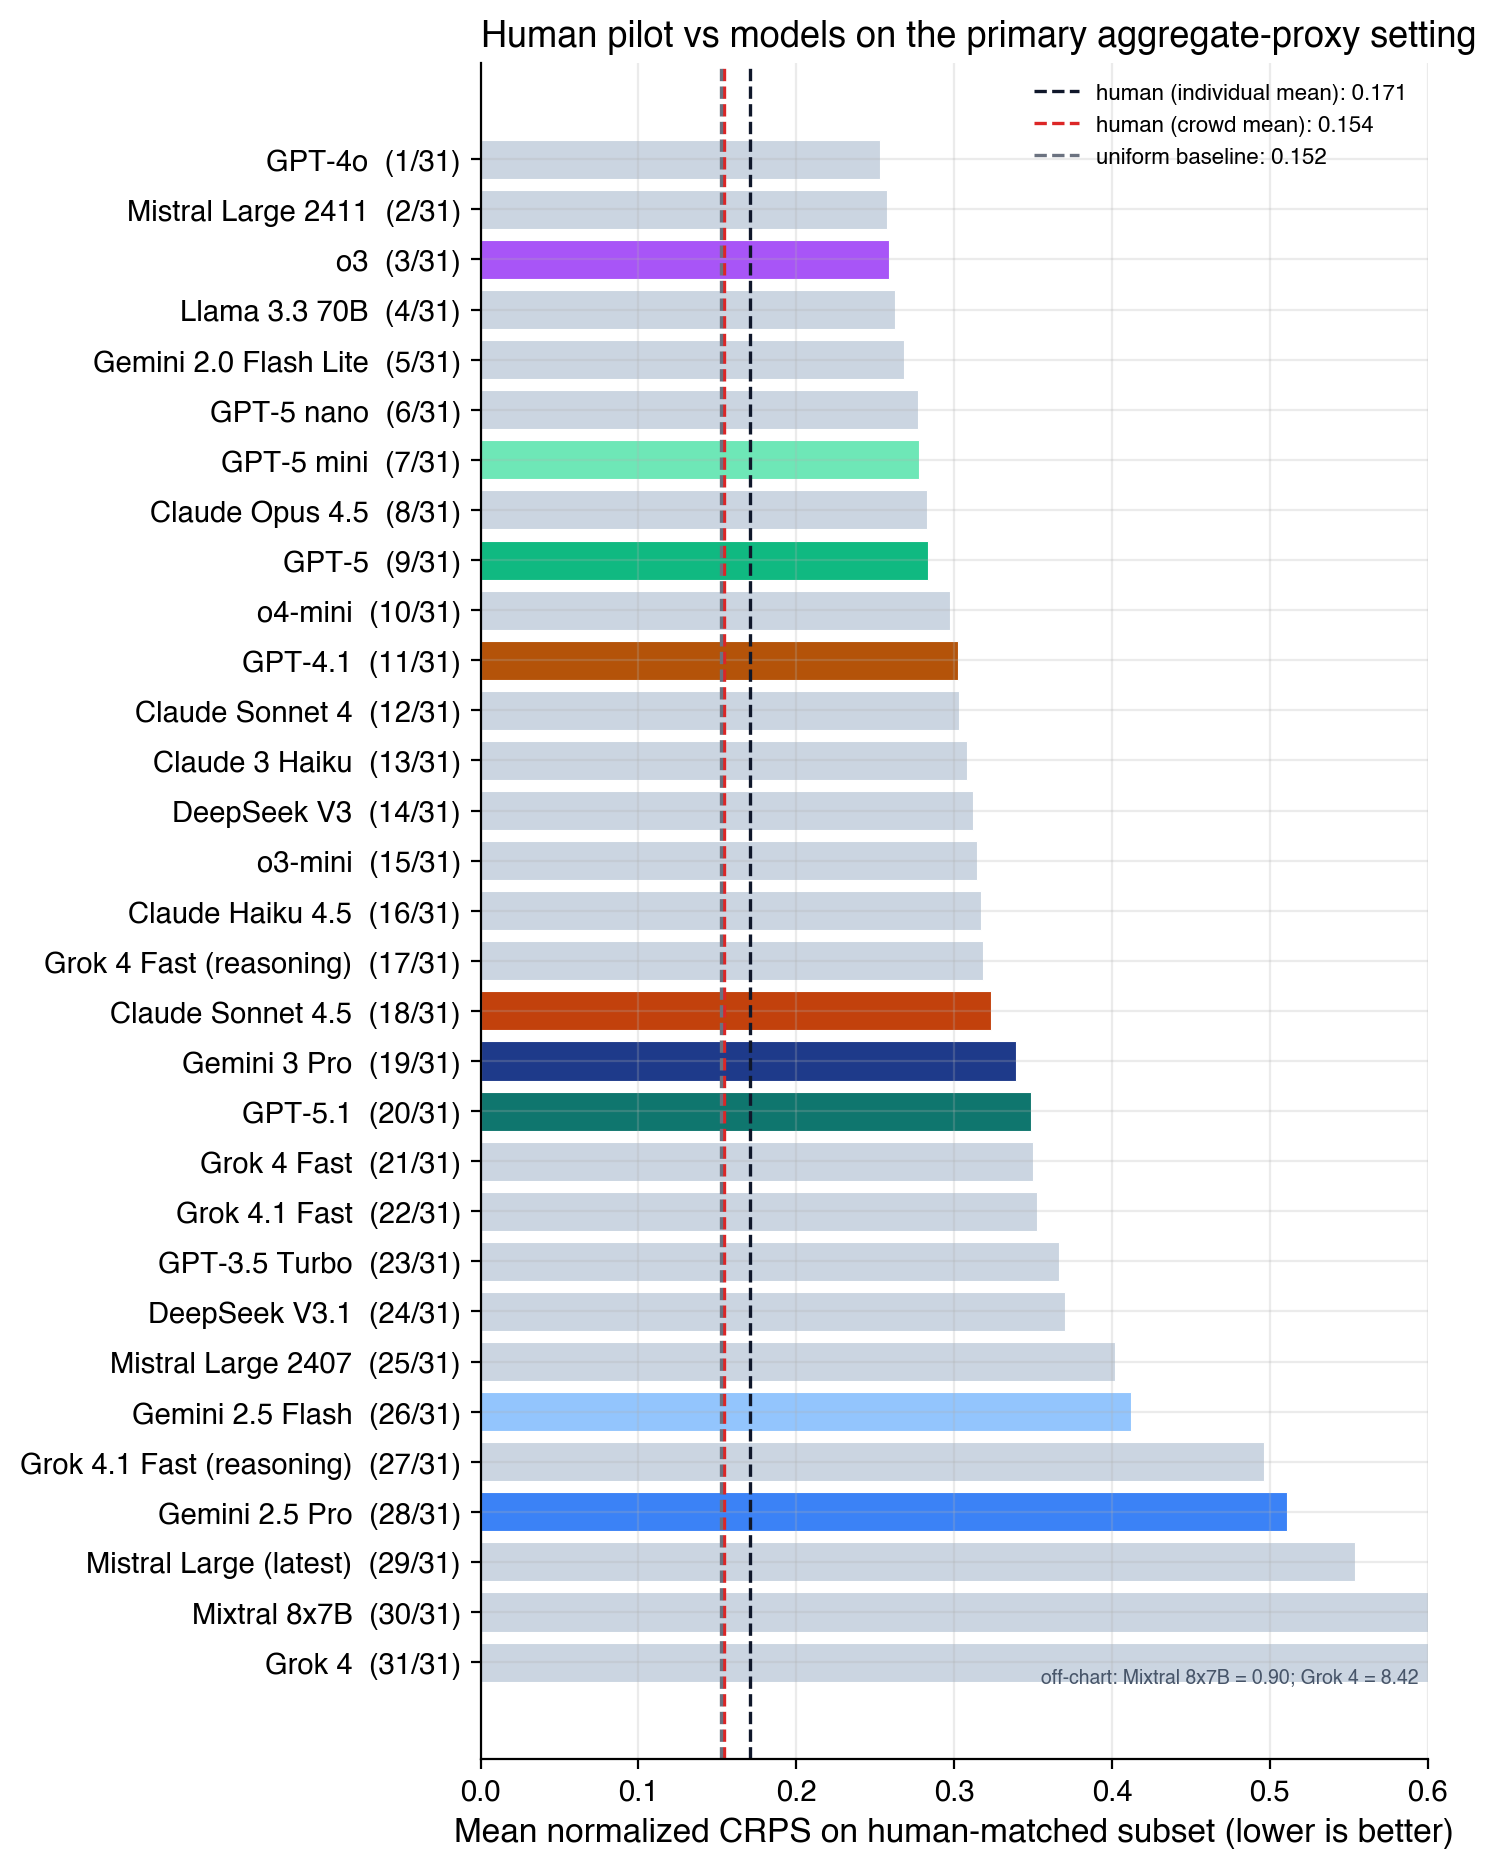
\includegraphics[width=.74\textwidth]{figA1_human_vs_models.png}
  \caption{Human pilot compared with models on the closest aggregate proxy: cities, technologies, and treasury at H1, H3, H4, and H6. The human pilot has 24 questions on 2 worlds; the model proxy uses the same template/horizon family across the larger model question set, so this is not a matched head-to-head comparison.}
  \label{fig:human-proxy}
\end{figure}

\section{Additional Validation Diagnostics}
\label{app:additional-validation}

The main text uses compact figures to keep the benchmark-design narrative readable. The full diagnostics below show the broader model set and several ways the benchmark can be sliced after forecasts are collected.

\begin{figure}[h]
  \centering
  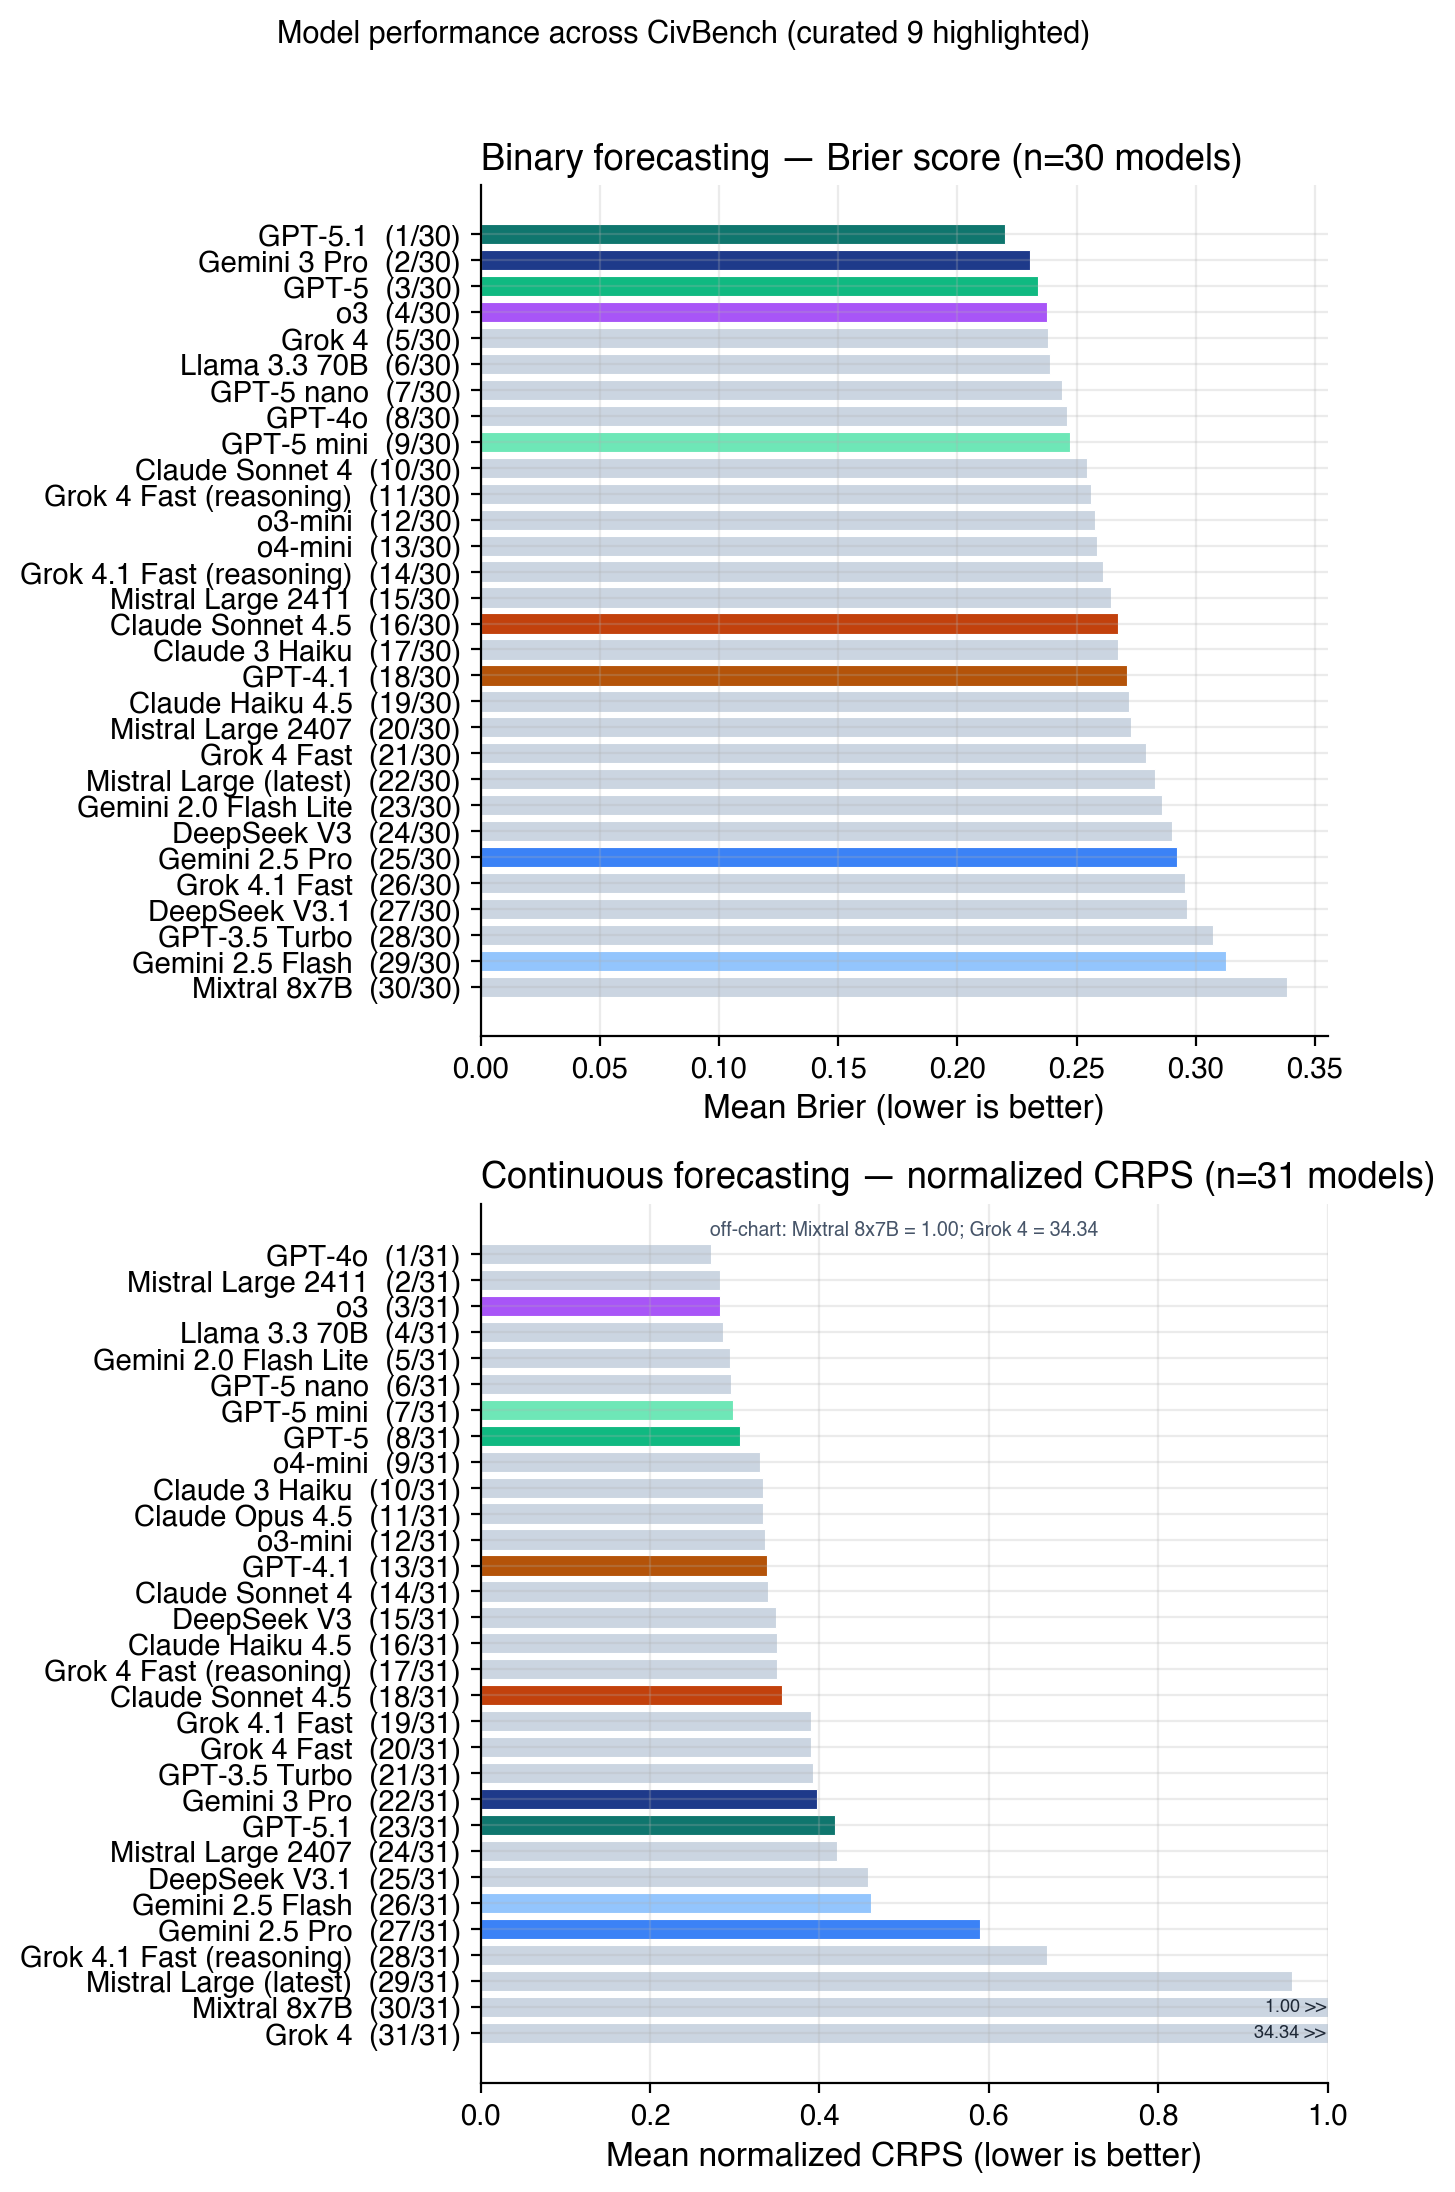
\includegraphics[width=.82\textwidth]{fig2_leaderboard.png}
  \caption{Full binary and continuous leaderboard. Curated models are highlighted, while additional models provide context for the compact validation figure in the main text.}
  \label{fig:full-leaderboard}
\end{figure}

\begin{figure}[h]
  \centering
  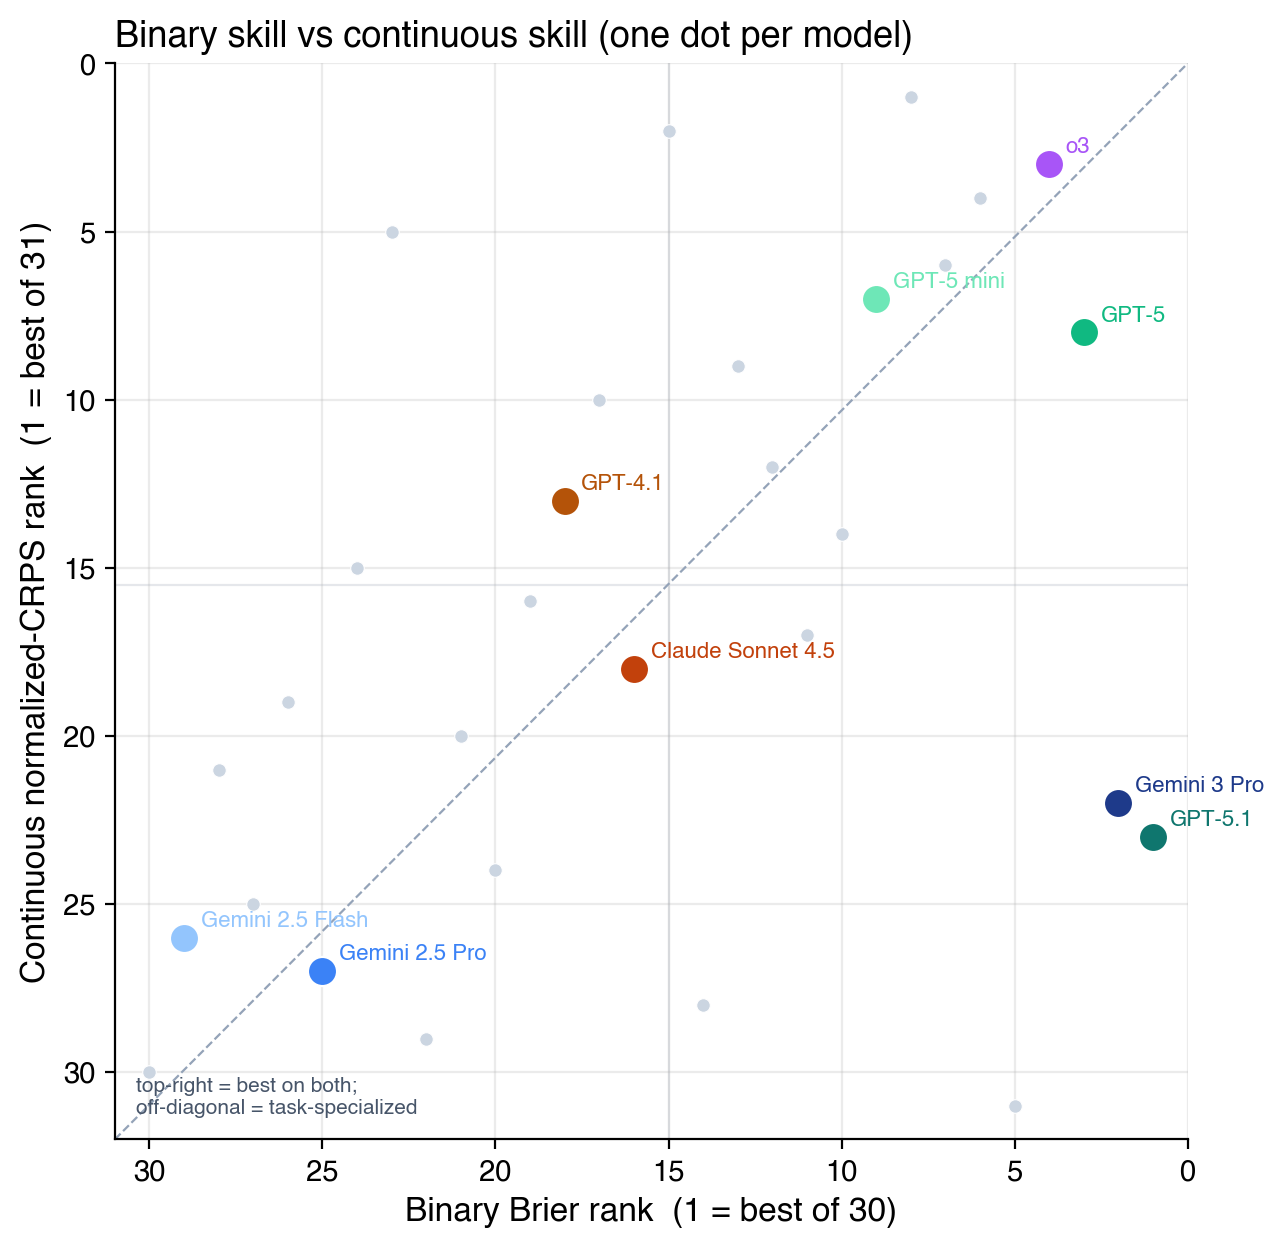
\includegraphics[width=.72\textwidth]{fig5_binary_vs_continuous.png}
  \caption{Binary and continuous performance are related but not identical. Some models rank well under Brier score while ranking lower under normalized CRPS, consistent with the benchmark measuring more than one forecasting skill.}
  \label{fig:binary-continuous}
\end{figure}

\begin{figure}[h]
  \centering
  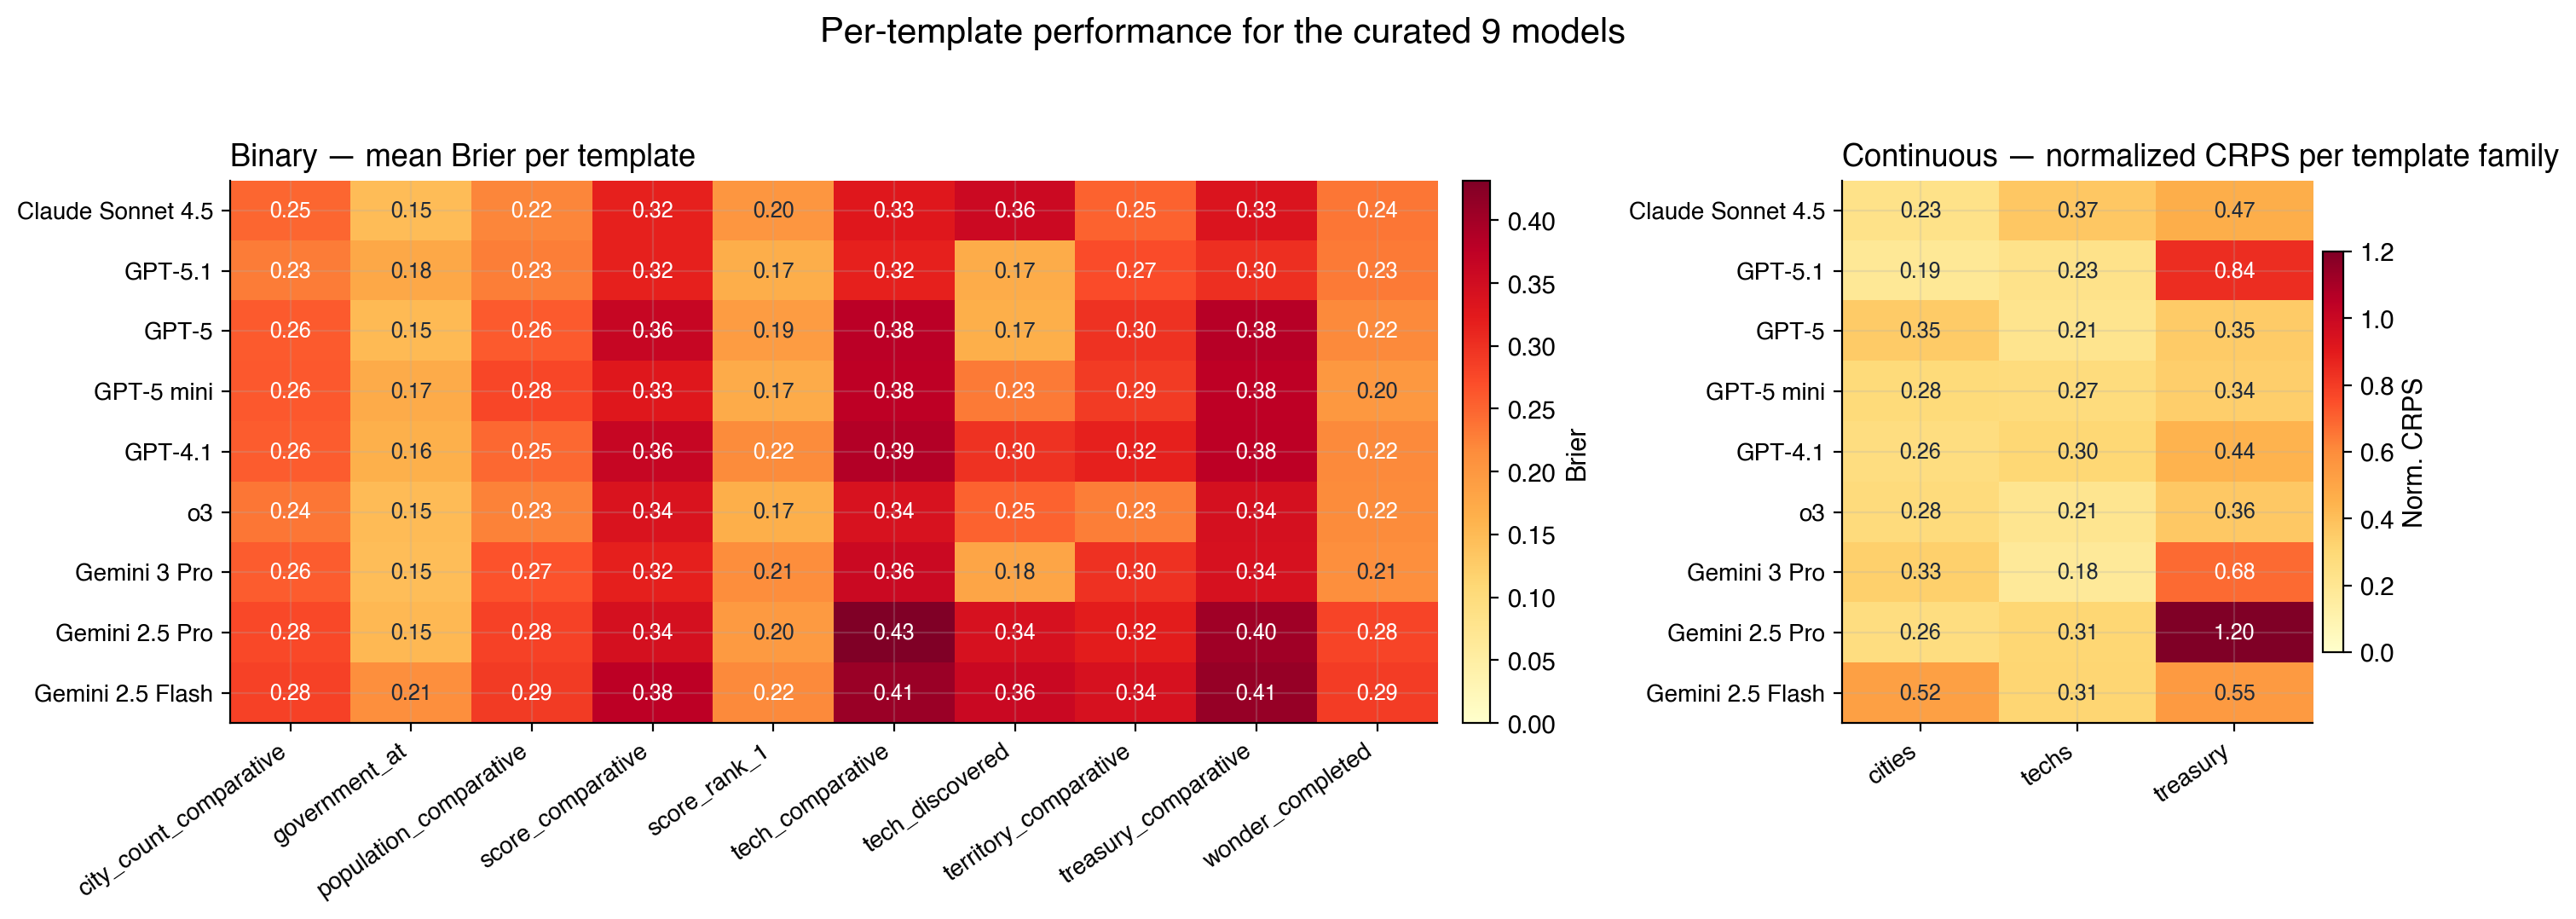
\includegraphics[width=\textwidth]{figA2_template_heatmap.png}
  \caption{Template and horizon slices expose heterogeneous difficulty. This is useful for separating predictable quantities, such as technologies, from quantities more exposed to disruption, such as treasury or city count.}
  \label{fig:template-heatmap}
\end{figure}

\begin{figure}[h]
  \centering
  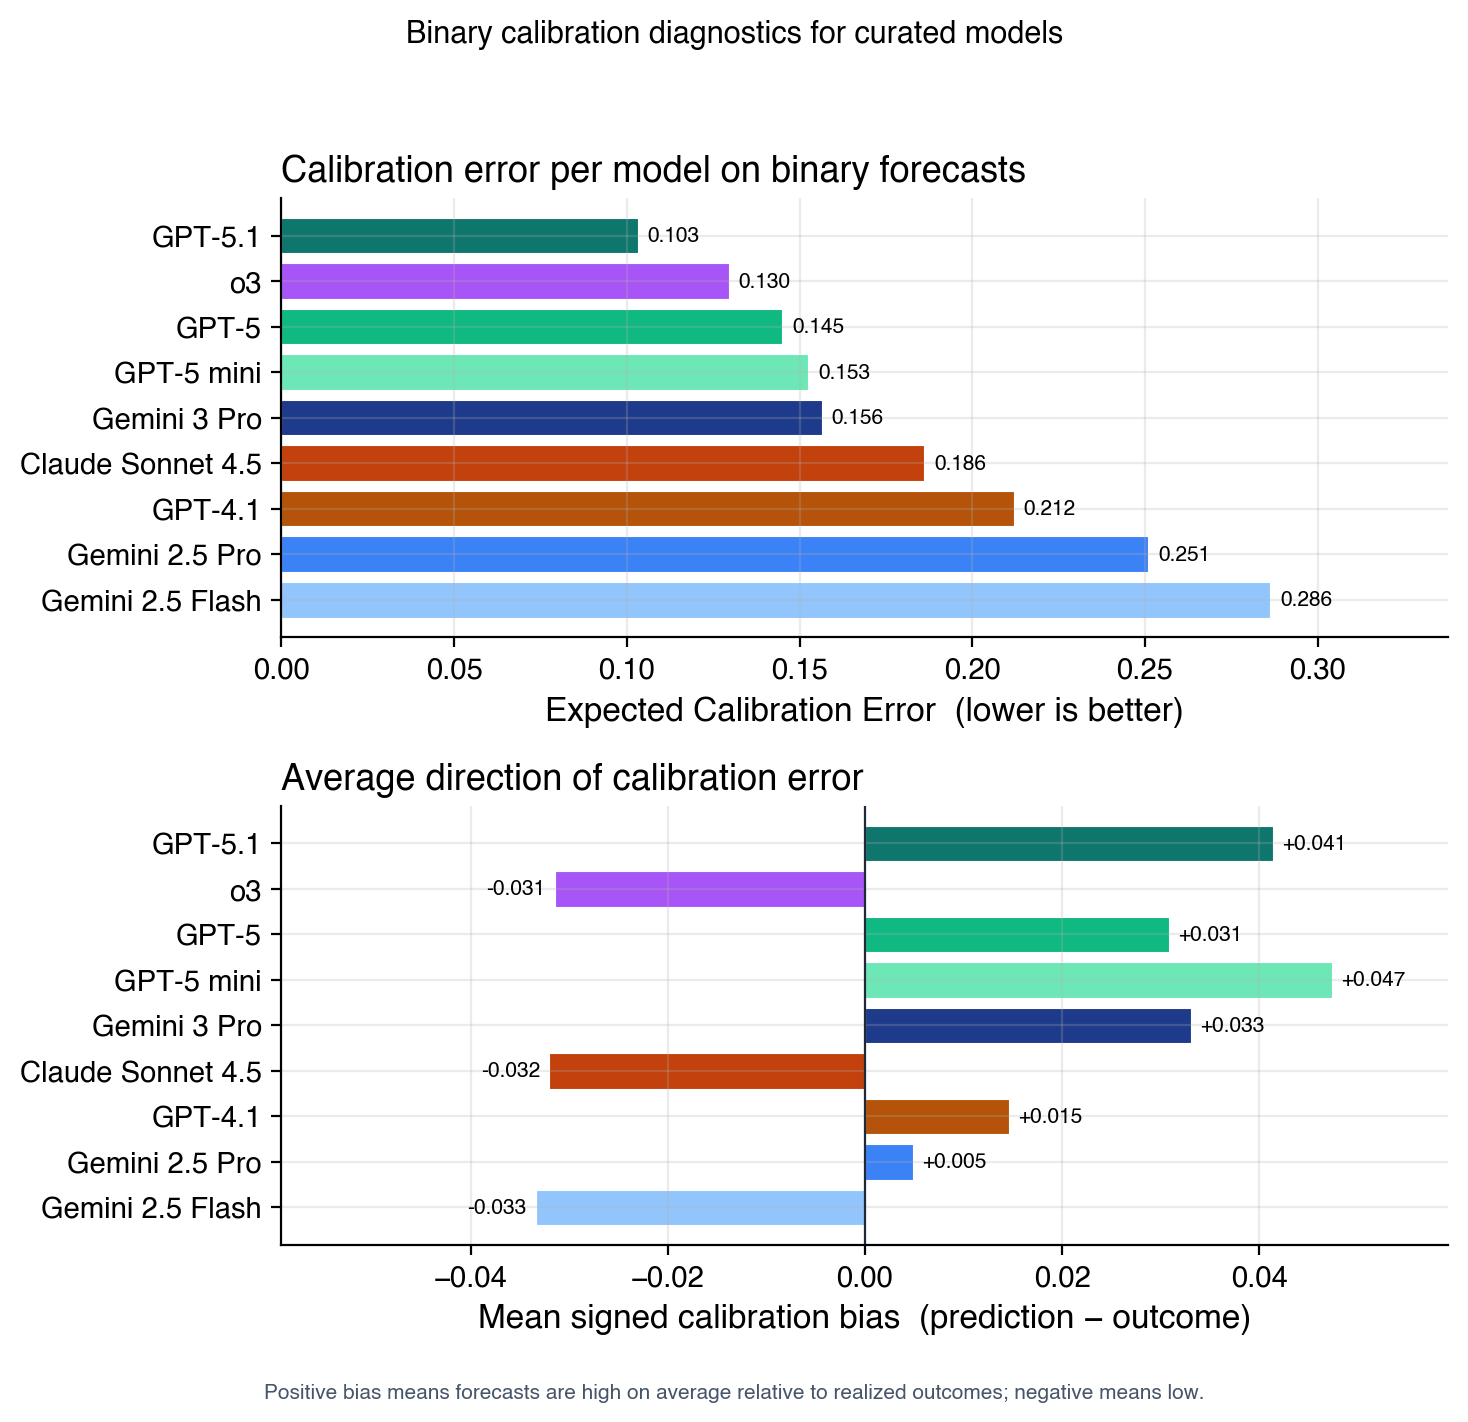
\includegraphics[width=.72\textwidth]{figA3_reliability.png}
  \caption{Binary calibration diagnostics for the curated model set. These diagnostics complement average Brier scores by showing whether errors are primarily calibration errors or discrimination errors.}
  \label{fig:binary-calibration}
\end{figure}

\section{Conditional Intervention Pilots}
\label{app:conditional-interventions}

The archived conditional pilot runs use two interventions: a government switch to Republic and a +500 treasury shock. For each intervention, we compare a model's baseline forecast against its conditional forecast on the intervention-world outcome. Positive intervention gain means that conditioning on the intervention moved the forecast closer to the forked-world ground truth. These runs are not a final intervention benchmark, but they demonstrate the paired-rollout machinery that real-world forecasting benchmarks usually cannot provide.

\begin{figure}[h]
  \centering
  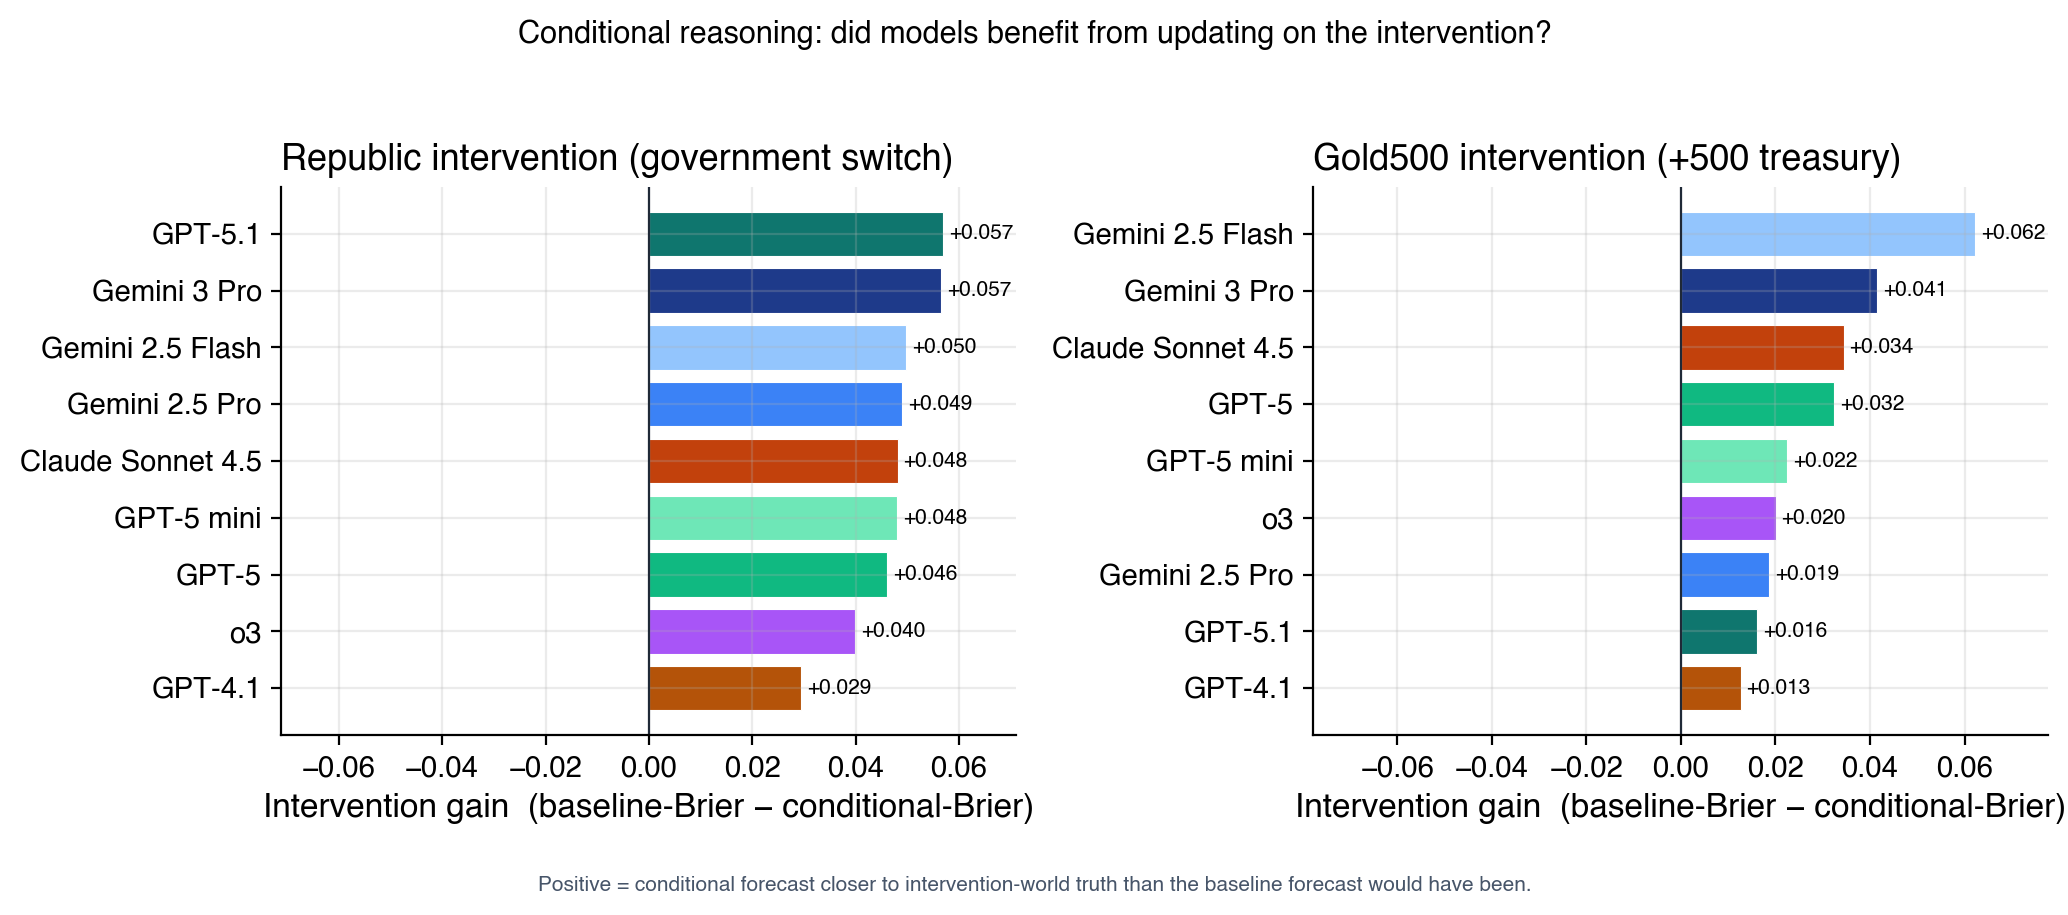
\includegraphics[width=.92\textwidth]{fig4_intervention_gap.png}
  \caption{Conditional intervention gains for Republic and +500 gold pilots. Positive values indicate that the conditional forecast was closer to the intervention-world outcome than the baseline forecast would have been.}
  \label{fig:intervention-gap}
\end{figure}

The appendix also includes a small placebo control for conditional phrasing. In an archived Opus 4.5 Republic pilot, replacing the intervention with a null conditional leaves performance near baseline, while the real intervention sharply worsens it. This is the clearest current evidence that the score shift is tied to intervention content rather than only to the presence of an ``if'' clause.

\begin{figure}[h]
  \centering
  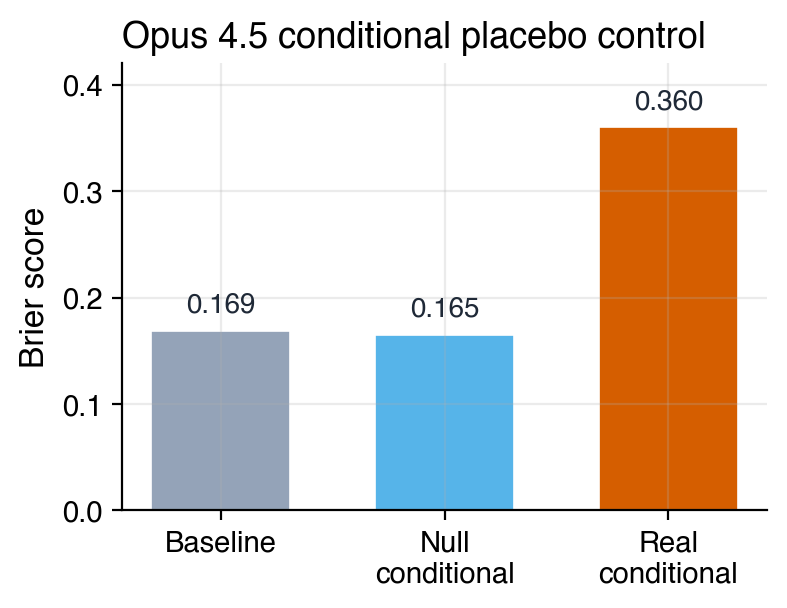
\includegraphics[width=.62\textwidth]{figA4_null_conditional.png}
  \caption{Placebo control for conditional framing in an Opus 4.5 Republic pilot. Replacing the intervention with a null conditional leaves Brier essentially unchanged from baseline, while the real intervention sharply degrades performance.}
  \label{fig:null-conditional}
\end{figure}

\section{Tail-Risk Diagnostic Example}
\label{app:tail-risk}

The same immediate-resolution substrate can support downstream studies of rare and disruptive outcomes. \Cref{fig:tail-risk} shows one example adapted from a companion anonymous analysis on the same CivBench continuous question family \citep{anonymous2026capability}: once many simulated worlds are sampled, the benchmark can expose systematic undercoverage of downside outcomes by horizon and template.

\begin{figure}[h]
  \centering
  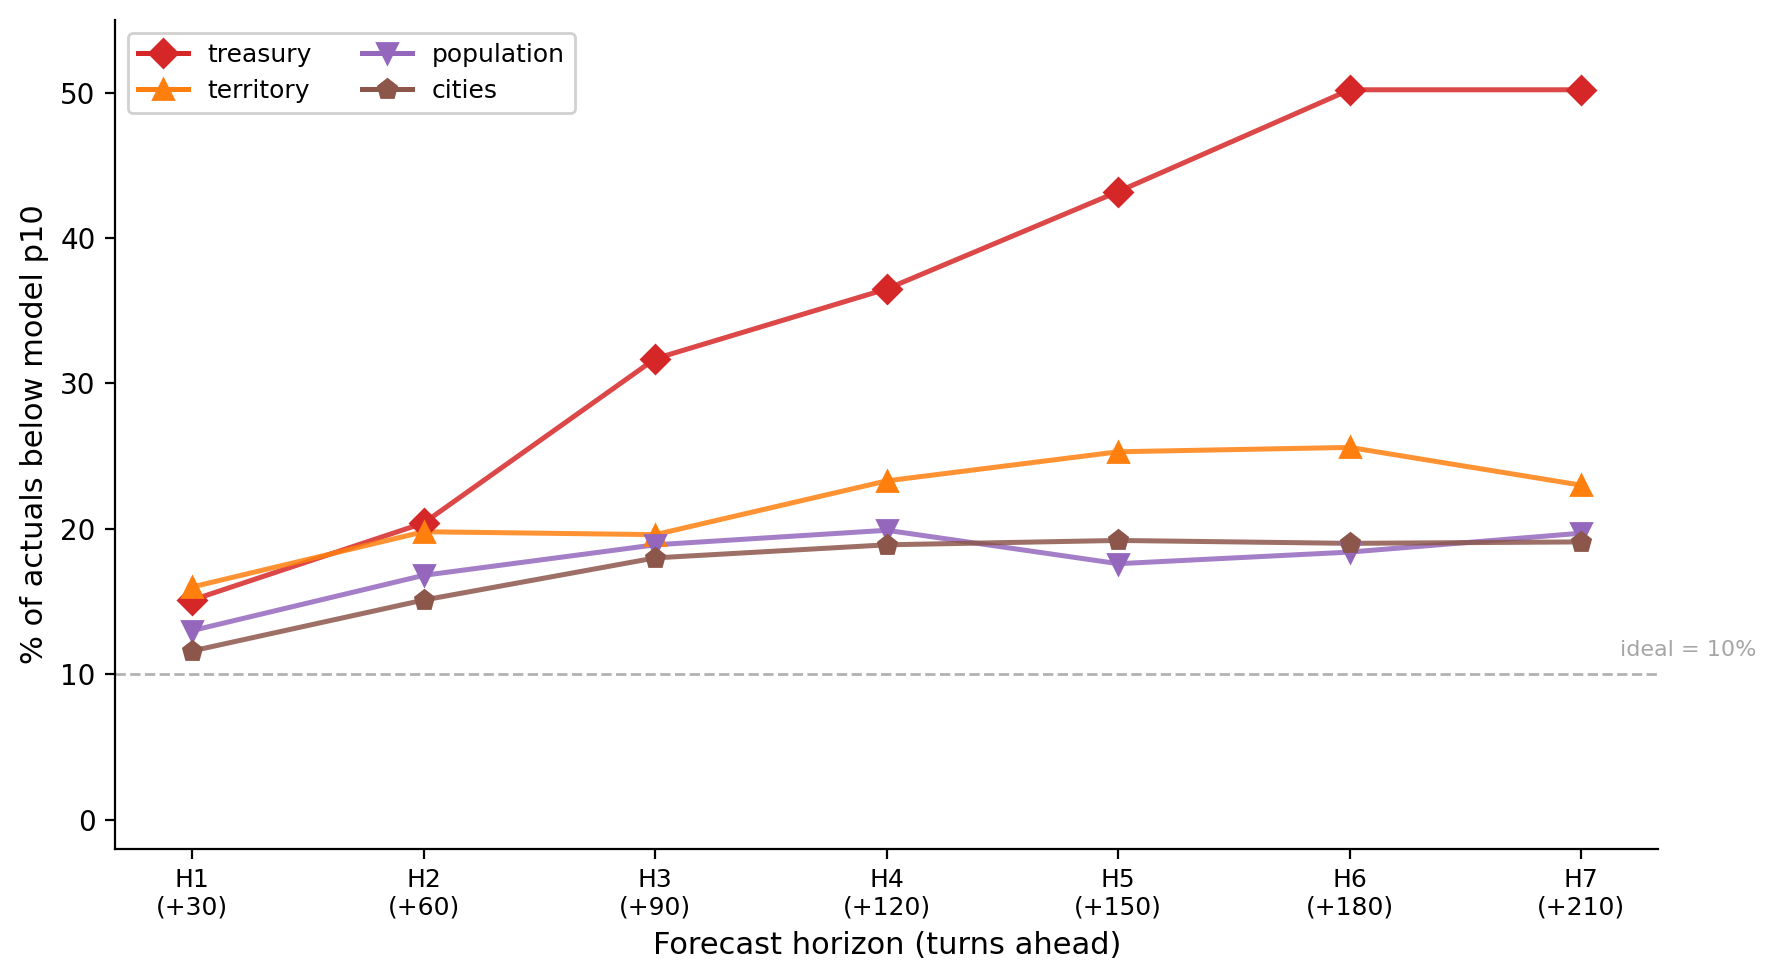
\includegraphics[width=.86\textwidth]{figA5_tail_risk.png}
  \caption{Example tail-risk diagnostic enabled by dense simulated-world sampling, adapted from a companion anonymous analysis on the same CivBench question family \citep{anonymous2026capability}. On disruptable continuous templates, the fraction of actuals falling below the model's stated p10 rises well above the nominal 10\% rate, with treasury reaching about 50\% by H6--H7.}
  \label{fig:tail-risk}
\end{figure}

\end{document}
